\documentclass{article}
\usepackage{graphicx,subfigure}
\begin{document}

\begin{figure}[!h]
  \centering
  \subfigure[TIF 1024 x 768 at scale = 0.33 Fig14 skin:hs]{
  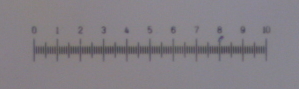
\includegraphics[scale=0.33]{figgradslide25xcrop.png}
  }\vfill
  \subfigure[JPG 2592 x 1944 at scale = 0.38 Fig18 fig:fibre3types] {
  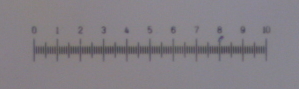
\includegraphics[scale=0.38]{figgradslide25xcrop.png}
  }\vfill
  \subfigure[JPG 2592 x 1944 at scale = 0.55 Fig13 fig:notwist] {
  
\includegraphics[scale=0.55]{mic25x2592x1944crop.jpg}
  }\vfill
  \subfigure[JPG 2592 x 1944 rot crop at scale = 0.15 Fig12 fig:twist] {
  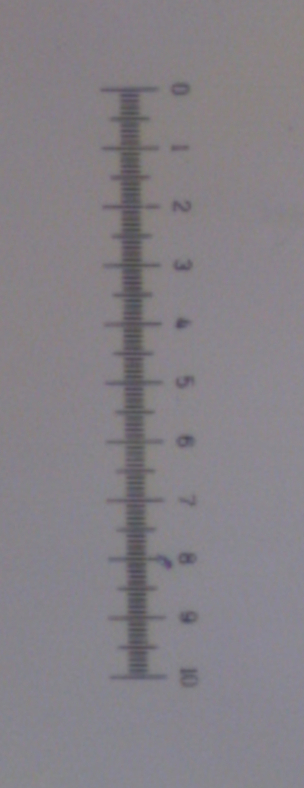
\includegraphics[scale=0.55,angle=90]{mic25x2592x1944rotcrop.jpg}
  }

% 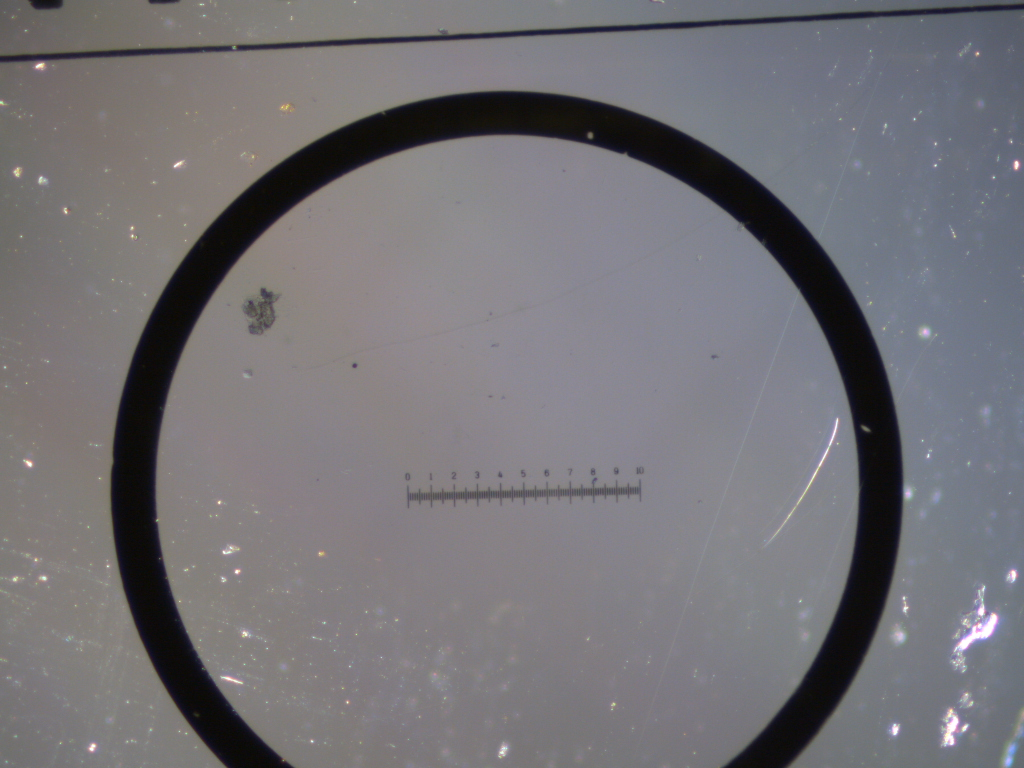
\includegraphics[scale=0.33]{figgradslide25x.png}
% 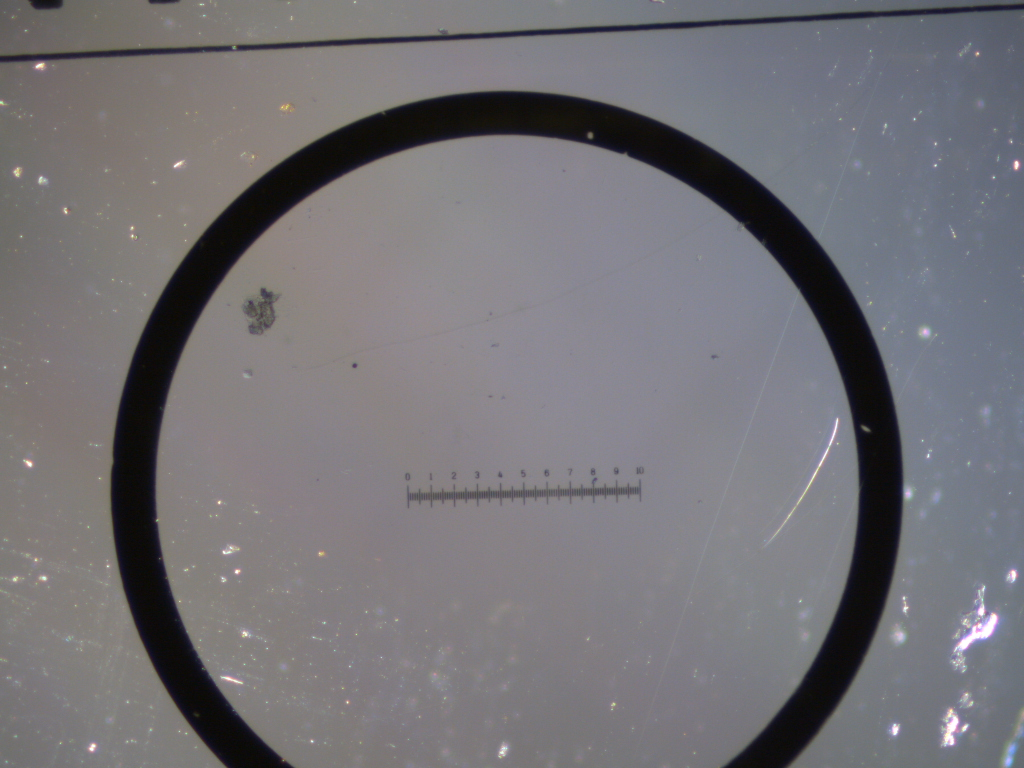
\includegraphics[scale=1.0]{figgradslide25x.png}

  \caption{Photomicrographs of a graduated slide at 25x microscope magnification, at various scale factors and resolutions, to match those of each of the text Figures.}
  \label{fig:gradslide25x}
\end{figure}

\end{document}

